% ------------------------------------------------------------------------- %
%  PLIK GENEROWANY AUTOMATYCZNIE przez apka/app.py (render_latex).
%  Nie edytować out.tex ręcznie — zmiany wprowadzać w apka/template.latex.
% ------------------------------------------------------------------------- %

\subsection{Analiza statystyczna}
\label{sub:statystyka}

Analizy wykonano w~języku Python (\texttt{pandas}, \texttt{NumPy},
\texttt{SciPy}). Przyjęto poziom istotności $\alpha = 0{,}05$ i~testy
dwustronne. Ze względu na porządkowy charakter skal (1--3 i~1--5) oraz
binarny charakter typowości smaku stosowano metody nieparametryczne
i~metody dla danych jakościowych. Każdy respondent oceniał wszystkie siedem
próbek.

\textit{Ślepy panel.} Dla każdej próbki obliczono odsetek ocen ,,smak
typowy'' z~95\% przedziałem Wilsona \cite{Wilson1927} i~sprawdzono testem
dwumianowym, czy różni się on od 0{,}5 (brak przewagi żadnej z~odpowiedzi).
Zdolność panelu do różnicowania próbek oceniono testem $Q$ Cochrana dla
typowości \cite{Cochran1950} oraz testem Friedmana dla ogólnej akceptacji
-- dla wszystkich siedmiu próbek oraz po wyłączeniu próbki o~skrajnie
wysokiej typowości.

\textit{Laboratoria.} Zgodność między trzema laboratoriami stosującymi
kwalifikator typowości wyrażono współczynnikiem $\kappa$ Fleissa
\cite{Fleiss1971} (interpretacja wg \cite{LandisKoch1977}) dla skali
binarnej (zastrzeżenie / brak zastrzeżenia) i~trzystopniowej (N / L / T).

\textit{Panel a~laboratoria.} Zbieżność rankingu próbek w~panelu
i~w~laboratoriach oceniono korelacją rang Spearmana ($n = 7$ próbek).
Próbki jednogłośnie zakwestionowane przez laboratoria porównano z~próbkami
bez zastrzeżeń na poziomie respondenta: dla każdej osoby obliczono różnicę
średniej typowości (oraz ogólnej akceptacji) obu grup próbek i~poddano ją
testowi Wilcoxona dla par \cite{Wilcoxon1945}; wielkość efektu wyrażono jako
$d$~Cohena dla danych sparowanych \cite{Cohen1988}. Zdolność pojedynczej
oceny panelisty do odtworzenia werdyktu większości laboratoriów oceniono
polem pod krzywą ROC (AUC) \cite{HanleyMcNeil1982} oraz odsetkami błędów
reguły ,,próbka nietypowa, gdy panelista uznał smak za nietypowy''.

%,,, -- %
\section{Wyniki}

\subsection{Charakterystyka panelu}

W~badaniu wzięło udział \textbf{138}~respondentów, którzy
łącznie wystawili 966~ocen (po 7~na osobę). Według dat
w~arkuszu panelu próbki oceniano w okresie maj-lipiec 2026.
Panel tworzyło 71~kobiet (51{,}4\%) i~64~mężczyzn
(46{,}4\%); dla 3~osób nie podano płci.
Najliczniejszą grupę wiekową stanowiły osoby poniżej 25.~roku życia
($n = 51$; 37\%), następnie osoby w~wieku
25--45 lat ($n = 37$; 26{,}8\%) i~46--65 lat
($n = 36$; 26{,}1\%); powyżej 65.~roku życia było
13~osób (9{,}4\%), a~1~osoba nie podała
wieku. Miód codziennie lub kilka razy w~tygodniu spożywało
44~osób (31{,}9\%), raz w~miesiącu
35 (25{,}4\%), a~okazyjnie
55 (39{,}9\%); 4~osoby
nie udzieliły odpowiedzi.

\subsection{Profil organoleptyczny próbek w~ślepym panelu}

Profil organoleptyczny siedmiu próbek przedstawiono w~tabeli~\ref{tab:lots}.
Średnia ogólna akceptacja wyniosła 3{,}261 (SD~1{,}241),
a~odsetek ocen ,,smak typowy dla miodu naturalnego'' -- 0{,}563.
Wyraźnie wyróżniała się próbka~P3 (typowość 0{,}905); typowość
pozostałych sześciu próbek mieściła się w~wąskim przedziale od 0{,}438
(P6) do 0{,}558 (P1).

\begin{table}[H]
\caption{Profil organoleptyczny próbek w~ślepym panelu konsumenckim.
\emph{Ocena} -- średnia ogólna akceptacja (1--5); \emph{Typowość} -- odsetek
ocen ,,smak typowy dla miodu naturalnego''; \emph{Słodycz}, \emph{Kwasowość},
\emph{Aromat} -- średnia na skali 1--3 (1~=~za słaba, 2~=~w~sam raz,
3~=~za silna); $n$ -- liczba odpowiedzi na pytanie o~typowość.\label{tab:lots}}
\begin{adjustwidth}{-\extralength}{0cm}
\begin{tabularx}{\fulllength}{lcCCCCC}
\toprule
\textbf{Próbka} & $\boldsymbol{n}$ & \textbf{Ocena} &
\textbf{Typowość} & \textbf{Słodycz} & \textbf{Kwasowość} & \textbf{Aromat} \\
\midrule
P1 & 138 & 3{,}37 & 0{,}558 & 2{,}07 & 1{,}77 & 1{,}69 \\
P2 & 137 & 3{,}04 & 0{,}496 & 2{,}06 & 1{,}77 & 1{,}81 \\
P3 & 137 & 3{,}92 & 0{,}905 & 2{,}20 & 1{,}89 & 2{,}06 \\
P4 & 137 & 3{,}15 & 0{,}540 & 2{,}12 & 1{,}82 & 1{,}82 \\
P5 & 136 & 3{,}16 & 0{,}515 & 2{,}33 & 1{,}89 & 2{,}08 \\
P6 & 137 & 3{,}07 & 0{,}438 & 2{,}26 & 1{,}87 & 2{,}04 \\
P7 & 137 & 3{,}11 & 0{,}489 & 2{,}23 & 1{,}81 & 1{,}85 \\
\bottomrule
\end{tabularx}
\end{adjustwidth}
\end{table}

Panel istotnie różnicował próbki zarówno pod względem typowości
($n = 136$ respondentów z~kompletem odpowiedzi;
$Q = 94{,}00$, $df = 6$, $p < 0{,}001$), jak i~ogólnej
akceptacji ($n = 129$; Friedman $\chi^2 = 55{,}35$, $p < 0{,}001$). Po wyłączeniu
P3 różnice między pozostałymi sześcioma próbkami nie były istotne ani dla
typowości ($Q = 6{,}35$, $df = 5$, $p = 0{,}274$), ani dla
ogólnej akceptacji ($\chi^2 = 7{,}95$, $p = 0{,}159$). Tylko dla
1 z~7~próbek (P3) odsetek ocen ,,typowy'' różnił się istotnie
od 0{,}5 (tabela~\ref{tab:panel_lab}).

\subsection{Ocena organoleptyczna w~laboratoriach}

Zakodowane werdykty trzech laboratoriów stosujących kwalifikator typowości
zestawiono w~tabeli~\ref{tab:panel_lab}, a~pełne, dosłowne opisy
-- w~tabeli~\ref{tab:interlab_opisy} (Załącznik~\ref{app:interlab_raw}).
Wszystkie trzy laboratoria uznały zapach lub smak próbek P6, P7 za
nietypowy dla miodu, żadne nie zgłosiło zastrzeżeń do próbek P3, P4, P5,
a~próbki P1 i~P2 zakwestionowało tylko jedno laboratorium. Pełną zgodność
na skali binarnej uzyskano dla 5 z~7~próbek
($\kappa = 0{,}60$, zgodność umiarkowana), a~na skali trzystopniowej
tylko dla 3 z~7~próbek ($\kappa = 0{,}33$,
zgodność słaba).

Czwarte laboratorium (metoda PN-88/A-77626) nie posługiwało się
kwalifikatorem typowości i~dla wszystkich siedmiu próbek orzekło ,,cechy
niejednoznaczne''. W~opisach wskazało zapach charakterystyczny dla oznak
fermentacji w~P1, P5 i~P6, zapach nienaturalny w~P2 i~landrynkowy w~P7
(tabela~\ref{tab:interlab_opisy}). Próbka~P5 nie budziła przy tym
zastrzeżeń żadnego z~trzech pozostałych laboratoriów, a~P1 -- dwóch z~nich.

\subsection{Zestawienie panelu z~wynikami laboratoriów}

\begin{table}[H]
\caption{Ślepy panel konsumencki a~ocena organoleptyczna trzech laboratoriów.
$n$ -- liczba odpowiedzi w~panelu; \emph{Typowość} -- odsetek ocen
,,smak typowy'' z~95\% przedziałem Wilsona; $p$ -- test dwumianowy względem 0{,}5.
Kody laboratoriów: T -- typowy, L -- lekko lub słabo typowy, N -- nietypowy
dla miodu (niższa z~ocen zapachu i~smaku). \emph{Zastrz.} -- liczba
laboratoriów z~oceną N.\label{tab:panel_lab}}
\begin{adjustwidth}{-\extralength}{0cm}
\begin{tabularx}{\fulllength}{lcCCCcccc}
\toprule
 & \multicolumn{4}{c}{\textbf{Ślepy panel}} &
\multicolumn{4}{c}{\textbf{Laboratoria}} \\
\cmidrule(lr){2-5}\cmidrule(lr){6-9}
\textbf{Próbka} & $\boldsymbol{n}$ & \textbf{Typowość} & \textbf{95\% CI} &
$\boldsymbol{p}$ & \textbf{1} & \textbf{2} & \textbf{3} & \textbf{Zastrz.} \\
\midrule
P1 & 138 & 0{,}558 & 0{,}47--0{,}64 & 0{,}201 & N & L & T & 1/3 \\
P2 & 137 & 0{,}496 & 0{,}41--0{,}58 & 1{,}000 & N & L & L & 1/3 \\
P3 & 137 & 0{,}905 & 0{,}84--0{,}94 & $<$0{,}001 & T & L & T & 0/3 \\
P4 & 137 & 0{,}540 & 0{,}46--0{,}62 & 0{,}393 & L & L & L & 0/3 \\
P5 & 136 & 0{,}515 & 0{,}43--0{,}60 & 0{,}797 & L & L & T & 0/3 \\
P6 & 137 & 0{,}438 & 0{,}36--0{,}52 & 0{,}171 & N & N & N & 3/3 \\
P7 & 137 & 0{,}489 & 0{,}41--0{,}57 & 0{,}864 & N & N & N & 3/3 \\
\bottomrule
\end{tabularx}
\end{adjustwidth}
\end{table}

Ranking próbek w~panelu był zbieżny z~rankingiem laboratoryjnym
(tabela~\ref{tab:panel_lab}, rysunek~\ref{fig:panel_lab}): korelacja
Spearmana między typowością w~panelu a~średnim kodem laboratoriów wyniosła
$\rho = 0{,}87$ ($p = 0{,}010$; dla ogólnej akceptacji
$\rho = 0{,}82$, $p = 0{,}024$). Po wyłączeniu
próbki~P3 korelacja przestała być istotna ($\rho = 0{,}79$,
$p = 0{,}059$). Większościowa odpowiedź panelu (typowość
$< 0{,}5$) pokryła się z~większościowym werdyktem laboratoriów dla
6 z~7~próbek.

\begin{figure}[H]
\begin{adjustwidth}{-\extralength}{0cm}
\centering
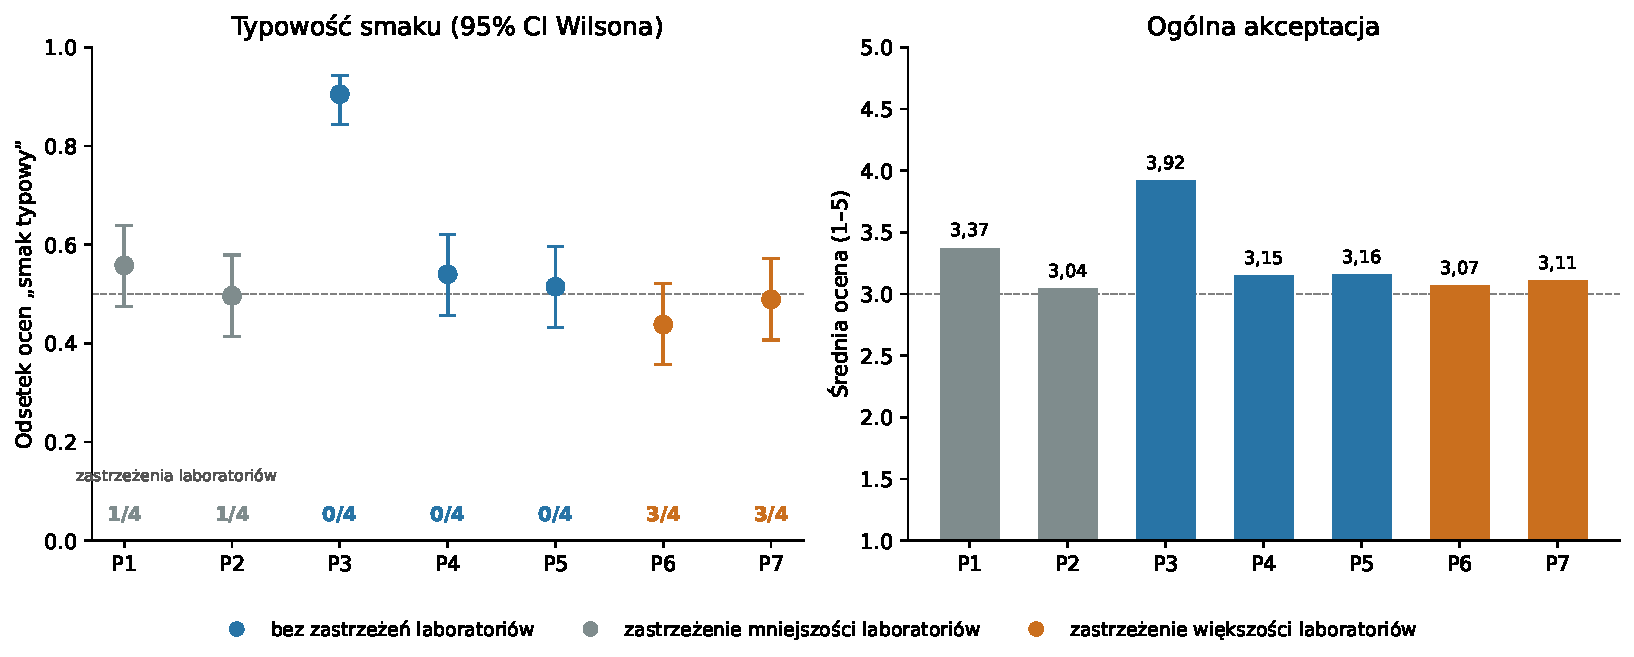
\includegraphics[width=16cm]{fig_panel_lab.pdf}
\end{adjustwidth}
\caption{Typowość smaku (punkty, 95\% przedział Wilsona) i~ogólna akceptacja
(słupki) siedmiu próbek w~ślepym panelu. Kolor oznacza werdykt laboratoriów:
niebieski -- brak zastrzeżeń, szary -- zastrzeżenie jednego laboratorium,
pomarańczowy -- zastrzeżenie wszystkich trzech; liczby u~dołu lewego panelu
-- liczba laboratoriów (z~trzech), które uznały zapach lub smak za nietypowy.
Linie przerywane -- 0{,}5 i~3.\label{fig:panel_lab}}
\end{figure}

Próbki jednogłośnie zakwestionowane przez laboratoria (P6, P7) uzyskały
w~panelu typowość 0{,}438 i~0{,}489 -- niższą od średniej, ale
nieodróżnialną od 0{,}5 ($p = 0{,}171$ i~$p = 0{,}864$). W~analizie
sparowanej typowość próbek bez zastrzeżeń laboratoryjnych (P3, P4, P5:
0{,}654) była wyższa niż próbek zakwestionowanych (P6, P7:
0{,}464); różnica wyniosła $\Delta = 0{,}189$ (95\% CI:
0{,}118--0{,}260; $p < 0{,}001$;
$d = 0{,}45$), a~dla ogólnej akceptacji $\Delta = 0{,}33$
punktu ($p = 0{,}002$) (rysunek~\ref{fig:contrast}). Po
wyłączeniu P3 różnica typowości spadła do $\Delta = 0{,}062$
i~przestała być istotna ($p = 0{,}144$).

\begin{figure}[H]
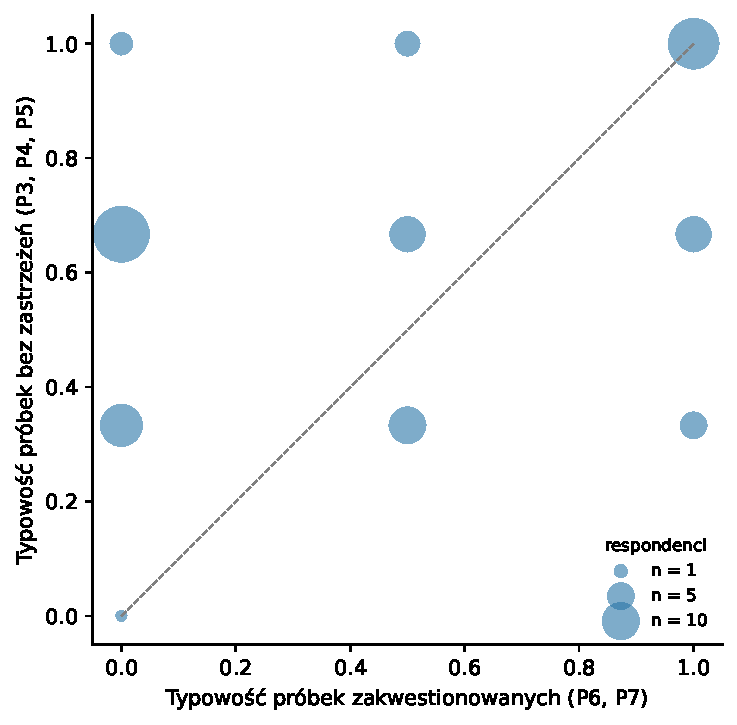
\includegraphics[width=8cm]{fig_contrast_lab.pdf}
\caption{Średnia typowość smaku próbek bez zastrzeżeń laboratoriów (oś~$y$)
i~próbek jednogłośnie zakwestionowanych (oś~$x$) dla każdego respondenta;
wielkość punktu -- liczba respondentów. Linia przerywana -- równość obu
ocen ($y = x$).\label{fig:contrast}}
\end{figure}

Pojedyncza ocena panelisty słabo odtwarzała werdykt większości laboratoriów
($\mathrm{AUC} = 0{,}570$, przy 0{,}5 dla zgadywania i~zwykle przyjmowanym
minimum 0{,}7 dla akceptowalnej dyskryminacji \cite{Hosmer2013}). Reguła ,,próbka nietypowa,
gdy panelista uznał smak za nietypowy'' wskazywałaby jako nietypowe
39{,}7\% ocen próbek, do których laboratoria nie miały zastrzeżeń,
i~uznawała za typowe 46{,}4\% ocen próbek przez nie
zakwestionowanych.

Panel zarejestrował natomiast cechę zbieżną z~częścią opisów
laboratoryjnych: słodycz oceniano jako ,,za silną'' najczęściej dla P5
(41{,}3\%), P6 (40{,}9\%) i~P7 (38{,}7\%), a~najrzadziej
dla P1 (22{,}1\%), P3 (22{,}6\%) i~P2 (24{,}1\%).
Czwarte laboratorium opisało jako ,,bardzo słodki'' smak P7, co zgadza się
z~oceną panelu, ale także smak P2, który panel rzadko oceniał jako zbyt
słodki.
